\chapter{Grundlagen}
\label{chap:grundlagen}
Container werden häufig als leichtgewichtige \glspl{acr-vm} beschrieben. Dies ist allerdings nicht ganz richtig. Wie in \fref{fig:containerVvm} zu erkennen, virtualisieren Container kein vollständiges \gls{acr-os}, sondern lediglich das benötigte Dateisystem. Dabei wird der Kernel des Hosts nicht virtualisiert, sondern lediglich mitverwendet. Dies macht Container deutlich leichtgewichtiger als \glspl{acr-vm}, isoliert allerdings weniger umfangreich als diese.
\begin{figure}[h]
		\subfigure[Container]{\missingfigure[figwidth=0.49\textwidth]{Container}}
		\hfill
		\subfigure[VM]{\missingfigure[figwidth=0.49\textwidth]{VM}}
		\caption{Virtualisierung durch \glspl{acr-vm} und Container}
		\label{fig:containerVvm}
\end{figure}

Dieses Kapitel behandelt alle benötigten Grundlagen, die zur Isolation eines Prozesses benötigt werden. Es werden vorhandene Standards wie die \gls{acr-oci} und benötigte Systemcalls wie \gls{acr-chroot} näher erläutert. Zudem wird beschrieben, wie die Isolation, die Container bieten, durch Systemmittel des Linuxkernels selber erreicht werden kann.
\section{Standards}
\label{sec:standards}

\subsection{App Container}
\label{sec:appc}
\todo{AppC einordnen appc $\to$  oci und cncf für Projekte die nicht in oci passen}
\subsection{Open Container Initiative}
\label{sec:oci}
Die \gls{acr-oci} ist eine Initiative, die seit 2015 unter der Linux Foundation agiert. Das Ziel der OCI ist es, einen offenen Standard für Container zu schaffen, sodass die Wahl der Container-Laufzeitumgebung nicht mehr zu Inkompatibilität führt. Dabei liegt der Fokus auf eine einfache, schlanke Implementierung \citep{OpenContainerInitiative}.

Die OCI arbeitet aktuell an zwei Spezifikationen. Die runtime-spec standardisiert die Laufzeitumgebung  von Containern. Dabei wird festgelegt, welche Konfiguration, Prinzipien und Schnittstellen Laufzeitumgebungen stellen müssen. Um die Umsetzung der runtime-spec zu fördern, stellt die OCI eine beispielhafte Implementierung durch runC.

Das zweite Projekt der OCI ist die image-spec. Dieses versucht einen Standard für \glspl{gls-image} zu definieren. Dabei plant die OCI nicht, vorhandene Image-Formate zu ersetzen, sondern auf diesen Aufzubauen und sie zu erweitern \citep{OpenContainerInitiative}.

\subsection{Cloud Native Computing Foundation}
\label{sec:cncf}
Die \gls{acr-cncf} beschäftigt sich im Gegensatz zur \gls{acr-oci} nicht nur mit Containern, sondern der kompletten \gls{gls-cloud}-Landscape. Projekte wie \gls{acr-k8} und Prometheus werden durch die \gls{acr-cncf} weiterentwickelt und publiziert \citep{CloudNativeComputingFoundation}. Da der Cloud-Native Entwicklungsprozess von Containern getragen wird, spielen Technologien wie containerd und rkt eine entscheidende Rolle für die \gls{acr-cncf}.

\begin{figure}[h]
	\begin{center}
		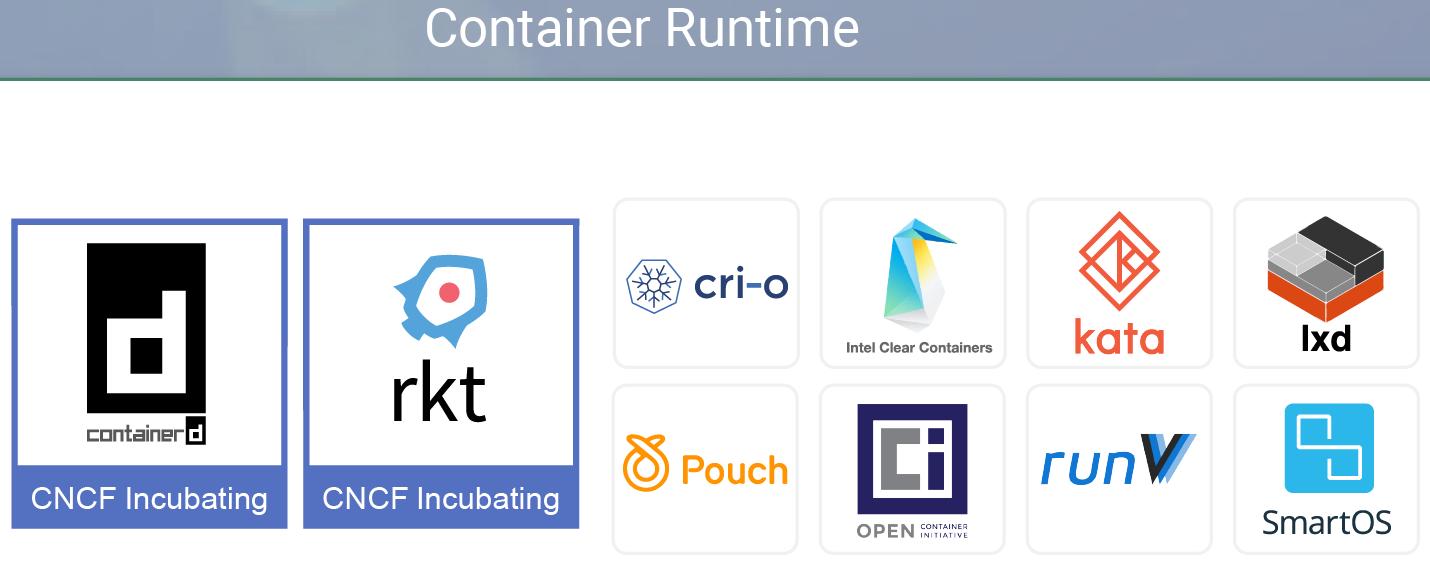
\includegraphics[scale=0.3]{bilder/cncf-container-landscape.png}
		\caption{CNCF Container Landscape \citep{CNCFCloudNativeInteractiveLandscape}}
		\label{fig:cncfContainerLandscape}
	\end{center}
\end{figure}

\todo{CoreOS Blog - Wo sitzt die CNCF zwischen appC und OCI}

\section{Funktionsweise}
\label{sec:funktionsweise}

Container isolieren einzelne Prozesse durch verschiedene Kernel Technologien, die im Folgenden erklärt werden sollen.
\subsection{Change Root}
\label{sec:chroot}
\Gls{acr-chroot} ist ein Unix Systemaufruf, der es erlaubt einen Prozess in einem anderen Wurzelverzeichnis auszuführen \citep{Chroot1LinuxManualPage}. Daraus folgt, dass der Prozess in einer eigenen Verzeichnisstruktur arbeitet und keine Änderungen am Dateisystem des Hosts machen kann. \Gls{acr-chroot} erlaubt somit die Isolierung des Dateisystems, die Container nutzen.

\subsection{Control Groups}
\label{sec:cgroups}
\glspl{acr-cgroup} dienen dazu, Systemressourcen für einzelne Prozesse zu limitieren. \todo{beschreibe cgroups, siehe \citep{ControlGroupV2}}

\subsection{Namespaces}
\label{sec:namespaces}

\subsection{Windows Hyper-V Container}
\label{sec:}

\todo{RunC Erklärung und ausführliche Beschreibung (libcontainer, runC, containerd ?, ...}

\section{Eigene Implementierung}
\label{sec:eigeneImpl}

Um die technischen Grundlagen zu vertiefen wurde eine eigene Container-Runtime entwickelt, die einen in Python geschriebenen Prozess isoliert und vom Hostsystem abschottet.